\begin{figure}[t]
  \centering
  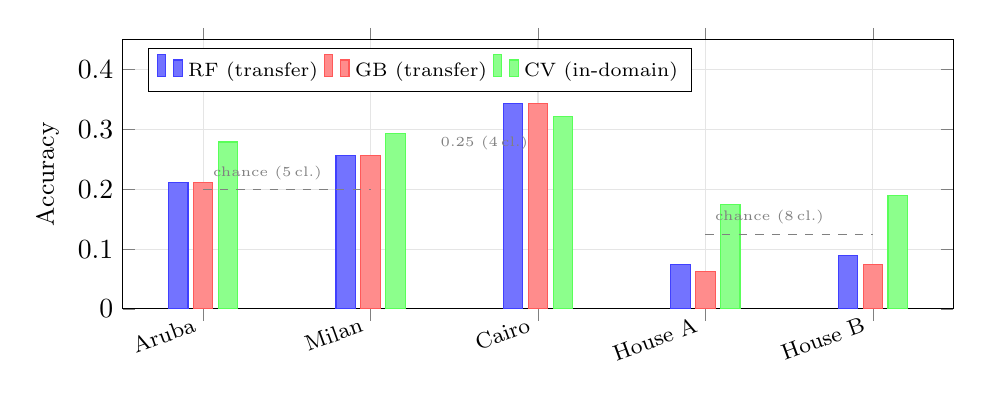
\begin{tikzpicture}
    \begin{axis}[
      ybar,
      width=\columnwidth,
      height=5cm,
      bar width=7pt,
      ylabel={Accuracy},
      ylabel style={font=\small},
      symbolic x coords={Aruba, Milan, Cairo, {House A}, {House B}},
      xtick=data,
      x tick label style={font=\footnotesize, rotate=20, anchor=east},
      ymin=0, ymax=0.45,
      ytick={0, 0.1, 0.2, 0.3, 0.4},
      grid=major,
      grid style={gray!20},
      enlarge x limits=0.12,
      legend style={at={(0.03,0.97)}, anchor=north west, font=\scriptsize,
                    legend columns=3},
      legend cell align=left,
    ]
    % Random Forest accuracy
    \addplot[fill=blue!55, draw=blue!75] coordinates {
        (Aruba,0.211) (Milan,0.256) (Cairo,0.344)
        ({House A},0.075) ({House B},0.089)
    };
    % Gradient Boosting accuracy
    \addplot[fill=red!45, draw=red!65] coordinates {
        (Aruba,0.211) (Milan,0.256) (Cairo,0.344)
        ({House A},0.063) ({House B},0.075)
    };
    % Cross-val on VESPER data (reference upper bound)
    \addplot[fill=green!45, draw=green!65] coordinates {
        (Aruba,0.279) (Milan,0.293) (Cairo,0.321)
        ({House A},0.175) ({House B},0.190)
    };
    \legend{RF (transfer), GB (transfer), CV (in-domain)}

    % Random chance reference lines
    \draw[gray, thin, dashed] (axis cs:Aruba,0.200) -- (axis cs:Milan,0.200);
    \node[font=\tiny, text=gray, anchor=south west] at (axis cs:Aruba,0.200) {chance (5\,cl.)};
    \draw[gray, thin, dashed] (axis cs:Cairo,0.250) -- (axis cs:Cairo,0.250)
      node[font=\tiny, text=gray, anchor=south east] {0.25 (4\,cl.)};
    \draw[gray, thin, dashed] (axis cs:{House A},0.125) -- (axis cs:{House B},0.125);
    \node[font=\tiny, text=gray, anchor=south west] at (axis cs:{House A},0.125) {chance (8\,cl.)};

    \end{axis}
  \end{tikzpicture}
  \caption{Zero-shot Sim2Real transfer accuracy across five real-world
  datasets.  Classifiers are trained on \sys{}-generated activity features
  and evaluated on held-out real data.  CASAS datasets (4--5 classes)
  achieve above-chance transfer; ARAS datasets (8 classes) present a
  harder challenge due to finer-grained categories.
  Dashed lines: uniform random baselines per class count.}
  \label{fig:sim2real}
\end{figure}
